\chapter{Ziel des Versuchs, Theoretische Grundlagen}

Das Rasterkraftmikroskop (AFM) sowie dessen Vorgänger, das Rastertunnelmikroskop (STM), gehören zum Gebiet der Rastersondenmikroskopen, bei denen Bilder einer Oberfläche nicht mit optischen oder elektronenoptischen Abbildung erzeugt wird, sondern mit durch Wechselwirkung einer Sonde mit der Probe. Mit dem Rasterkraftmikroskop können, im Gegensatz zum Rastertunnelmikroskop, nicht elektrisch leitfähige Oberflächen in nm-Bereich abgebildet werden.

\section{Funktionsprinzip des AFM}
Eine nanoskopisch kleine Spitze, die in einen geringen Abstand über oder auf der Probe positioniert wird, tastet zeilenweise die Beschaffenheit einer Oberfläche in einem definierten Raster ab. Diese Nadel ist an einer Blattfeder, dem Cantilever, befestigt und wird von Pizokristallen über die Oberfläche bewegt. Wenn die Spitze über die Oberfläche geführt wird, verbiegt sich der Cantilever relativ zum Höhenprofil der Probenoberfläche, aufgrund der wirkenden Kräfte zwischen der Messspitze und der Probe. Ein Laserstrahl ist auf die Rückseite des Cantilevers gerichtet und wird von dort auf einen positionssensitiven Photodetektor, die Viersegmentphotodiode, reflektiert. Verbiegt sich nun der Cantilever, so registieren die Photodioden die Positionsverschiebungen der Laserreflexion, wodurch Rückschlüsse auf die Oberflächeneigenschaften der Probe geschlossen werden können.\\
Um eine hohe Auflösung zu erzielen, sollte eine feine Spitze mit einem kleinen Spitzenradius verwendet werden, allerdings sind solche Spitzen empfindlicher. Üblicherweise sind sowohl die Spitze als auch der Cantilever aus Silizium oder Siliziumnitrid, es werden aber auch Diamant oder andere Materialien verwendet. Um bei beispielsweise rauen Oberflächen mit kleinen Strukturen die gesamten Informationen der Topographie zu erhalten, sollte das Aspektverhältnis der Spitze groß sein. Hierzu werden Kohlenstoff-Nanoröhrchen auf die Silizumspitze aufgebracht, damit auch feine Spitzen mechanisch stabil sind. Die Form des Cantilevers ist ein Balken oder ein Dreieckshebel. Je nach zu untersuchenden Oberfläche variiert die Federkonstante. Daher sollte die Federkonstante klein sein, um die Probenoberfläche nicht zu beschädigen und trotzdem kleine Kraftwechselwirkungen zu erfassen. Zudem ist es auch wichtig, dass die Resonanzfrequenz hoch genug ist, um eine Einkopplung mechanischer und akustischer Schwingungen zu vermeiden.
\begin{figure}[H]
    \centering
    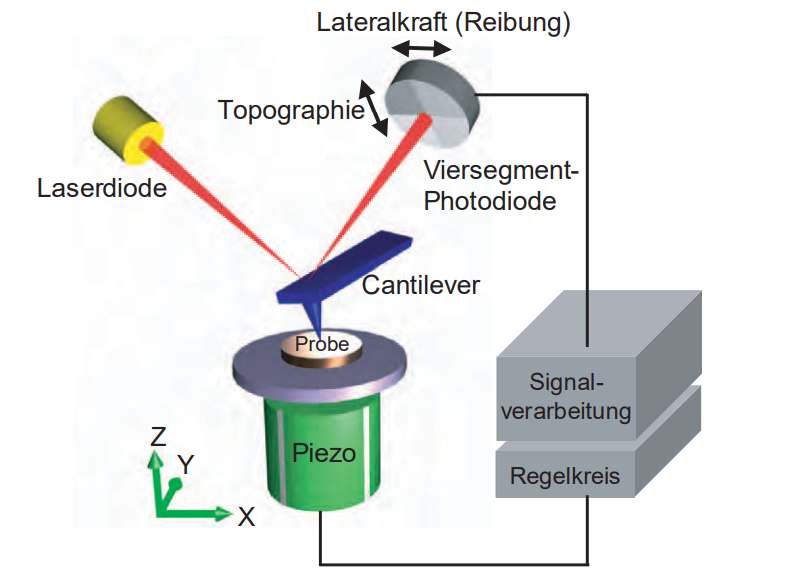
\includegraphics[width=70mm,scale=0.35]{Rasterkraftmikroskop/include/Rasterkraftmikroskop.PNG}
    \caption{Schematische Darstellung des Rasterkraftmikroskops} 
    \label{fig:Rasterkraftmikroskop}
\end{figure}


\section{Auflösungsbegrenzung}
\label{chap:aufloesung}
Für das maximale Auflösungsvermögen bei optischen Mikroskopen gilt nach dem Abbe-Kriterium:
$$x_\text{min}=\frac{\lambda}{n\text{sin}\phi}~.$$
Hierbei ist $x_\text{min}$ der kleinste noch auflösbare Abstand, $\lambda$ die Wellenlänge des Lichts und $n$ der Brechungsindex. $n\text{sin}\phi$ ist die nummerische Apertur. Während bei optischen Mikroskopen die Wellenlänge das Auflösungsvermögen begrenzt, ist es bei Rasterkraftmikroskopen die Feinheit der Spitze, also deren Radius und Aspektverhältnis. Wie in der folgenden Abbildung \ref{fig:Auflösungsbegrenzung,Spitze} zu sehen ist, 
\begin{figure}[H]
    \centering
    \includegraphics[width=110mm,scale=0.5]{Rasterkraftmikroskop/include/Auflösungsbegrenzung,Spitze.PNG}
    \caption{Oberflächenabbildung mit einer stumpfen und einer scharfen Spitze} 
    \label{fig:Auflösungsbegrenzung,Spitze}
\end{figure}
wird eine feine Spitze benötigt, um auch die kleineren Details einer Oberfläche zu erfassen. Dafür sollte der Abstand der Oberflächentopographien größer sein als der Spitzenradius. Ist dies nicht der Fall und der die Oberflächentopographie hat die Form eines Deltapeaks, so ist die Abbildung der Spitze um 180° gedreht. Verfälschungen des Messsignals aufgrund von geometrischen Effekten werden Spitzenartefakte genannt. Nach einer Topographiemessung müssen die Scans daher auf Artefakte geprüft werden, um keine Fehlinterpretationen zu erhalten.


\section{Piezoelektrischer Effekt}
Wie schon beim Funktionsprinzip des Rasterkraftmikroskops erwähnt werden Piezoelemente genutzt, um die Spitze über der Probe zu bewegen. Der piezoelektrische Effekt ermöglicht eine Feinverstellung der Spitze im Subangstömbereich.  \\
Allgemein wird zwischen direktem und indirektem piezoelektrischen Effekt unterschieden. Beim direkten Piezoeffekt bewirkt eine Krafteinwirkung in piezoelektrischen Materialien, dass Ladungsträger verschoben werden und so ein Dipol erzeugt wird. Es wird also eine Spannung erzeugt, die über das Material abgegriffen werden kann. Der umgekehrte Effekt wird als indirekter oder auch inverser Piezoeffekt bezeichnet. Hier wir eine Spannung an das piezoelektrische Material angelegt, wodurch der Piezokristall verformt wird. Allerdings geschieht dies erst nach einer zeitlichen Verzögerung, was auch als \dq creep \dq bezeichnet wird.  \\
Zur feinen Positionierung der Spitze wird ein Scannerröhrchen aus piezoelektrischen Material verwendet. Oft sind dies ferroelektrische Keramiken. Zur lateralen Positionierung sind an der Außenseite der Röhre sind vier Metallelektroden angebracht. Die z-Positionierung erfolgt über eine Ringelektrode an der Innenseite des Röhrchens.
\\
Neben der Feinverstellung durch Ausnutzung des piezoelektrischen Effekts, erfolgt die Grobverstellung meist über Mikrometerschrauben, die von Hand oder über Schrittmotoren betätigt werden.


\section{Betriebsmodi}
\subsection{Contact Mode}
Wird das Rasterkraftmikroskop im Contact Mode betrieben, steht die Messspitze in direktem Kontakt mit der zu analysierenden Oberfläche. Es wir das Lichtzeigerprinzip verwendet. Hierbei wird an jedem Rasterpunkt die Ablenkung des Cantilevers detektiert. Dieses Messverfahren kann geregelt und ungeregelt ablaufen.\\
\\
Der ungeregelte Modus wird auch Constant Height Modus genannt. Hier wird die Spitze über der Probe nicht nachgeregelt. Verbiegt sich der Cantilever aufgrund der Topographie der Probenoberfläche, ändert sich auch die Position des auf den Canitlever gerichteten Laserstrahls, der auf eine Viersegmentphotodiode reflektiert wird. An allen Segmenten der Photodiode kommt es daraufhin zu einer 
Spannungsänderung. Die Lichtanteile zwischen den oberen und den unteren Segmenten des Photodiodenfeldes sind nun verschoben. Beim Scan wird die Spannungsdifferenz (T-B-Signal) aufgezeichnet, welche ein Maß für die Lichtzeigerbewegung, also der Verbiegung des Cantilevers, ist. Neben Normalkräften, die zur Verbiegung des Cantilevers führen, treten auch Reibungskräfte auf, die zu einer Torsion des Cantilevers führen. Im Falle einer Torsion kann die Differenzspannung zwischen den nebeneinanderliegenden Photodioden (L-R-Signal) gemessen werden. Die Signale durch Verbiegung und Torsion sind gleichzeitig messbar und nicht komplett unabhängig voneinander. Wird ein Scan in Vorwärts- und Rückwärtsrichtung druchgeführt, so ergibt sich bei Reibungsbildern eine Hystereseschleife, wodurch eine Unterscheidung zwischen den Rasterbildern durch Reibungs- und Topographieeffekte möglich ist.
Da die Verbiegung des Cantilevers begrenzt ist, eignen sich glatte und harte sowie Oberflächen mit geringer Rauigkeit.\\

Um zu vermeiden, dass der Cantilever bei größeren Unebenheiten abbricht, kann die Messung im Constant Force Modus durchgeführt werden. Dabei wird immer wieder die Höhe der Spitze nachgeregtelt, sodass das Photodiondensignal konstant, also die Kraft auch die Spitze gleich bleibt. 


\subsection{Non-Contact Mode}
Für beispielsweise empfindliche und weiche Proben kann die Messung im Tapping Mode durchgeführt werden. Bei diesem Modus tippt der Cantilever auf die Probenoberfläche. Mittels eines Piezokristalls, an den eine Wechselspannung angelegt wird, wird der Cantilever in Schwingung nahe der seiner Eigenschwingung versetzt und in die Nähe der Probe gebracht. Hervorgerufen durch Wechselwirkung zwischen Probe und Cantilever, ändern sich die effektiven Federkonstanten bevor die Spitze die Probe berührt. Dementsprechend ändern sich auch die Resonanzfrequenz und die Schwingungsamplitude. Folglich fungiert der Cantilever als gedämpfter harmonischer Oszillator.\\
Ein Vorteil des Non-Contact Mode ist die geringe Krafteinwirkung auf die Probe. Dadurch kommt es zu weniger Zerstörungen der Probenoberfläche, wodurch Verfälschungen des Messsignals vermieden werden. Jedoch birgt dieses Messprinzip auch Nachteile. Es könne keine Reibungskräfte gemessen werden. Zudem ist die laterale Auflösung schlechter und die Messgeschwindigkeit langsamer im Vergleich zum Contact Mode.


\section{Kräfte zwischen Körpern}
Beim Annähern der Spitze an die Probe kommt es zu attraktiven und repulsiven Wechselwirkungen. Wegen der komplexen Geometrie bei der Rasterkraftmikroskopie müssen die auftretenden Kräfte als ein komplexes Vielteilchensystem betrachtet werden. 

\subsection{Van-der-Waals (VdW) Kräfte}
VdW Kräfte sind attraktive Kräfte und entstehen durch Dipol-Dipol-Wechselwirkung zweier Moleküle. Diese Kräfte dominieren die Wechselwirkung bei nichtmagnetischen und elektrisch neutralen Molekülen. Als Annahme können die VdW Kräfte aufsummiert werden. Über die Hamakerintegration kann die VdW Kraft zwischen zwei makroskopischen Körpern berechnet werden. Dabei gilt
$$F_\text{VdW}=-\frac{Hr}{6z^{2}}~.$$
$r$ ist der Radius einer Kugel, die sich im Abstand $z$ über einer glatten Oberfläche befindet. $H$ ist die materialspezifische Hamakerkonstante, die die Wechselwirkung zwischen makroskopischen Körpern beschreibt. Hier kann sie als konstant angenommen werden. Ist zwischen zwei Körpern Luft, so hat H einen Wert von $H=18,65 \cdot 10^{-20}\,$J. Sind die zwei Körper stattdessen durch Wasser getrennt, so hat ist $H=9,7 \cdot 10^{-20}\,$J. Für Letzteres mit einem Spitzenradius von $r=10\,$nm im Abstand $z=1\,$nm ergibt sich eine VdW Kraft von $F_\text{VdW}=1,6 \cdot 10^{-10}\,$N.

\subsection{Kapillarkräfte}
Aufgrund von Adsorbatschichten, diese sind mehrere Nanometer dicke Wasserfilme auf einer Oberfläche, entstehen bei Messungen an der Luft Kapillarkräfte. Zwischen Spitze und Probe setzen sich Wassertröpfchen fest, wodurch es zur Miniskusausbildung kommen kann. Dieser übt eine langreichweitige, attraktive Kraft auf die Spitze aus. Die Maximalkraft ist durch 
$$F_\text{Kapillar,max}=-4\pi R\sigma$$
mit dem Spitzenradius $R$ und der Oberflächenspannung $\sigma$ des Adsorbats gegeben. Für die Annahme, dass der Spitzeraidus wieder $R=10\,$nm beträgt und $\sigma=0,074\,\frac{\text{N}}{\text{m}}$ für Wasser, ergibt sich eine maximale Kapillarkraft von $F_\text{Kapillar,max}=9,3\cdot 10^{-9}\,$N.

\subsection{Repulsive Kräfte}
Repulsive Kräfte sind kurzreichweitig. Bei Annäherung der Spitze und der Oberfläche und somit deren Molekülen, überlappen sich deren Elektronenorbitale. Nach dem Pauli-Prinzip können Elektronen nicht denselben Energiezustand besetzen, weshalb sie zu energetisch höheren Orbitalen gehen. Dadurch erhöht sich die potentielle Energie. Der Potentialverlauf kann als $\frac{1}{z^{12}}$ Proportionalität angenommen werden. Bei großen Abständen zwischen Spitze und Probe kann die repulsive Kraft vernachlässigt werden. Bei einem Abstand von $1\,\mathring{\text{A}}$ beträgt die Kraft einige $10^{-8}\,$N.

\subsection{Lennard-Jones-Potential}
Die Zusammenfassung von repulsiven und attraktiven Anteilen liefert das Lennard-Jones-Potential
$$V(z)=4\epsilon\left(\left(\frac{\sigma}{z}\right)^{12}-\left(\frac{\sigma}{z}\right)^{6}\right)~,$$
dabei sind $\epsilon$ und $\sigma$ empirische Konstanten.
\begin{figure}[H]
    \centering
    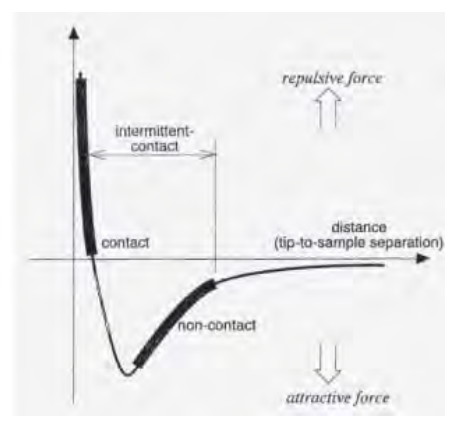
\includegraphics[width=60mm,scale=0.5]{Rasterkraftmikroskop/include/Lennard-Jones-Potential.PNG}
    \caption{Lennard-Jones-Potential} 
    \label{fig:Lennard-Jones-Potential}
\end{figure}

\section{Kraft-Abstands-Kurven}
\begin{figure}[H]
    \centering
    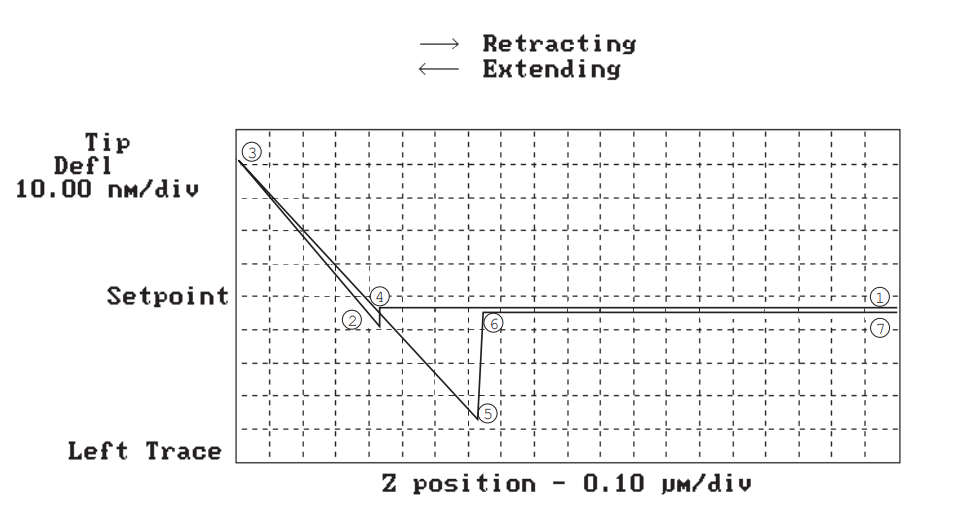
\includegraphics[width=130mm,scale=0.7]{Rasterkraftmikroskop/include/Kraft-Abstands-Kurve.PNG}
    \caption{Kraft-Abstands-Kurve} 
    \label{fig:Kraft-Abstands-Kurve}
\end{figure}
Mit Kraft-Abstands-Kurven können Aussagen über die Abstandsabhängigkeit der Kräfte und ihrer Stärke zwischen der Spitze und der Probe getroffen werden. Zuerst wird die Spitze der Probe genähert bis sie deren Oberfläche berührt und dann wird die Spitze wieder entfernt. Währenddessen wird die Verbiegung des Cantilevers aufgezeichnet. Eine solche Kurve ist in Abbildung \ref{fig:Kraft-Abstands-Kurve} zu sehen. Am Punkt 1 wird die Spitze der Probe genähert, sind jedoch noch nicht in Kontakt, weshalb noch keine Cantileververbiegung gemessen wird. Punkt 2 wird als \dq snap in\dq bezeichnet. Hier ist zu erkennen, dass ab einen gewissen Abstand zwischen Spitze und Probe die attraktiven Kräfte die Cantileverrückstellkraft überwiegen, wodurch der Cantilever sich abrupt nach unten biegt. Wird der Cantilever der Oberfläche weiter genähert, so befindet er sich zunächst wieder in seiner Ruhelage. Dies ist in Punkt 4 dargestellt. Hier sind repulsive und attraktive Kräfte gleich groß. Beim weiteren Annähern überwiegen schließlich die repulsiven Kräfte und der Cantilever wird nach oben verbogen. Dieser Bereich würde bei einer harten Oberfläche linear verlaufen, da sich hier die Oberfläche nicht elastisch verformt. In Punkt 3 wird die Spitze wieder von der Probe entfernt und die attraktiven und repulsiven Kräfte befinden sich im Gleichgewicht. Wird der Abstand nun weiter vergrößert, so überwiegen in Punkt 5, welcher auch als \dq snap off \dq bezeichnet wird, die Rückstellkräfte des Cantilevers und die Spitze entfernt sich schlagartig von der Oberfläche. Anschließend ist der Cantilever wieder unausgelenkt (Punkt 6). Die Ausprägung der Hysterese zwischen snap in und snap off wird maßgeblich von den Kapillarkräften bestimmt. Aus diesem Grund ist bei Messungen im Ultrahochvakuum oder in Flüssigkeiten die Hysterese sehr viel dünner, da der Adsorbatfilm sehr dünn oder sogar nicht vorhanden ist. \\
Nach dem Hookschen Gesetz gilt für die Auflagekraft $F_\text{n}$ des Cantilevers auf der Probenoberfläche
$$F_\text{n}=c_\text{n}S\Delta U_\text{T-B}~,$$
dabei ist $c_\text{n}$ die normale Federkonstante, $S$ die Sensitivität der Photodetektors in $\frac{\text{nm}}{\text{V}}$ und $\Delta U_\text{T-B}$ das Differenzsignal der Photodiode. Das Differenzsignal des nicht ausgelenkten Cantilevers kann als Kraftnullpunkt definiert werden. Aus der inversen Steigung des elastischen Bereichs der Kurve, kann dann die Sensitivität betimmt werden. Grundsätzlich ist die normale Federkonstante angegeben. Sie kann aber auch aus den geometrischen Daten berechnet werden.
$$c_\text{n}=\frac{E\omega t^{t}}{4l^{3}}$$
wobei $E$ das Elasitzitätsmodul, $\omega$ die Breite, $t$ die Dicke und $l$ die Länge ist. Typische Werte der Auflagekräfte liegen im Bereich $10^{-10}$ und $10^{-7}\,$N.
